\documentclass[11pt,compress,t,notes=noshow, aspectratio=169, xcolor=table]{beamer}

\usepackage{../../style/lmu-lecture}
% Defines macros and environments
% This file is included in slides and exercises

% Rarely used fontstyle for R packages, used only in 
% - forests/slides-forests-benchmark.tex
% - exercises/single-exercises/methods_l_1.Rnw
% - slides/cart/attic/slides_extra_trees.Rnw
\newcommand{\pkg}[1]{{\fontseries{b}\selectfont #1}}

% Spacing helpers, used often (mostly in exercises for \dlz)
\newcommand{\lz}{\vspace{0.5cm}} % vertical space (used often in slides)
\newcommand{\dlz}{\vspace{1cm}}  % double vertical space (used often in exercises, never in slides)
\newcommand{\oneliner}[1] % Oneliner for important statements, used e.g. in iml, algods
{\begin{block}{}\begin{center}\begin{Large}#1\end{Large}\end{center}\end{block}}

% Don't know if this is used or needed, remove?
% textcolor that works in mathmode
% https://tex.stackexchange.com/a/261480
% Used e.g. in forests/slides-forests-bagging.tex
% [...] \textcolor{blue}{\tfrac{1}{M}\sum^M_{m} [...]
% \makeatletter
% \renewcommand*{\@textcolor}[3]{%
%   \protect\leavevmode
%   \begingroup
%     \color#1{#2}#3%
%   \endgroup
% }
% \makeatother


\title{Interpretable Machine Learning}
% \author{LMU}
%\institute{\href{https://compstat-lmu.github.io/lecture_iml/}{compstat-lmu.github.io/lecture\_iml}}
\date{}

\begin{document}

% Set style/preamble.Rnw as parent.
\newcommand{\vertiii}[1]{{\left\vert\kern-0.25ex\left\vert\kern-0.25ex\left\vert #1 
    \right\vert\kern-0.25ex\right\vert\kern-0.25ex\right\vert}}
% Load all R packages and set up knitr

% This file loads R packages, configures knitr options and sets preamble.Rnw as 
% parent file
% IF YOU MODIFY THIS, PLZ ALSO MODIFY setup.Rmd ACCORDINGLY...

% Defines macros and environments
 \newcommand{\titlefigure}{figure/AEturtle.jpg} 
\newcommand{\learninggoals}{
\item Understand the definition of ADEs 
\item Understand first methods that generate ADEs
\item Discuss potential causes of ADEs and standard defenses against them}

\lecturechapter{\Large{Local Explanations: Adversarial Examples}}
\lecture{Interpretable Machine Learning}

% ------------------------------------------------------------------------------

\begin{frame}[c]{Adversarial Machine Learning}
\begin{itemize}
    \item What happens if a computer system gets an erroneous input?
    \item Even worse:\\ What happens if someone feeds in a malicious input on purpose to attack a system?
    \item[$\leadsto$] \textbf{Robustness} is important to ensure a safe service!
    \medskip
    \item \textbf{Adversarial ML} studies the robustness of machine learning (ML) algorithms to malicious input
    \item Two different kinds of attacks:
    \begin{itemize}
        \item \textbf{Evasion attacks} mislead an employed ML model with manipulated inputs (our focus)
        \item \textbf{Data Poisoning}: Malicious inputs to the training dataset
    \end{itemize}
    \end{itemize}
\end{frame}

\begin{vbframe}[c]{Adversarial Examples}
%The inputs by which evasion attacks can be conducted are called \textbf{Adversarial Examples (ADEs)}
\begin{itemize}
    \item \textbf{Informal Definition}: An ADE is an input to a model that is deliberately designed to "fool" the model into misclassifying it
    \item Even possible with low generalization error
    \item Both deep learning models (e.g., CNNs) and classical ML can be vulnerable to such attacks
    \item ADEs created from a real data observation $\xv$ can be indistinguishable from $\xv$ by a human observer 
    \item Since the model misclassifies this input, it does not seem to have a real understanding of the underlying concepts of the provided inputs
\end{itemize}
\end{vbframe}

\begin{vbframe}{Examples: Model-Attacks \citebutton{Gong \& Poellabauer 2018}{https://arxiv.org/pdf/1803.09156.pdf}}

\begin{columns}[totalwidth=\textwidth]

\begin{column}{0.6\textwidth}

\begin{figure}[h]
\centering
  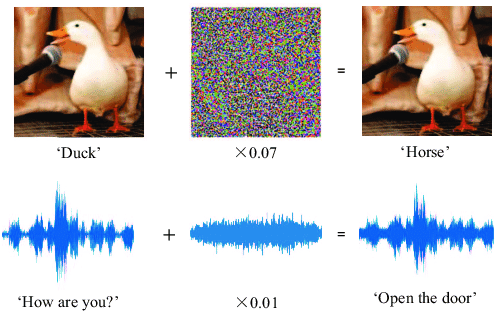
\includegraphics[width=1\linewidth]{figure/AEduckSound.png}
  \label{fig:mnist}
\end{figure} 

\end{column}

\begin{column}{0.4\textwidth}

    \vspace{3em}
    \begin{itemize}
        \item Is this a duck or a horse?
        \item Small (hard-to-see) noise can change the prediction
    \end{itemize}

\end{column}

\end{columns}

\end{vbframe}

\begin{vbframe}[c]{Examples: Image Data \citebutton{Eykholt et al. (2018)}{https://arxiv.org/pdf/1807.07769.pdf}  \citebutton{Athalye et al. (2018)}{https://arxiv.org/pdf/1707.07397.pdf}}
\begin{figure}[h]
\centering
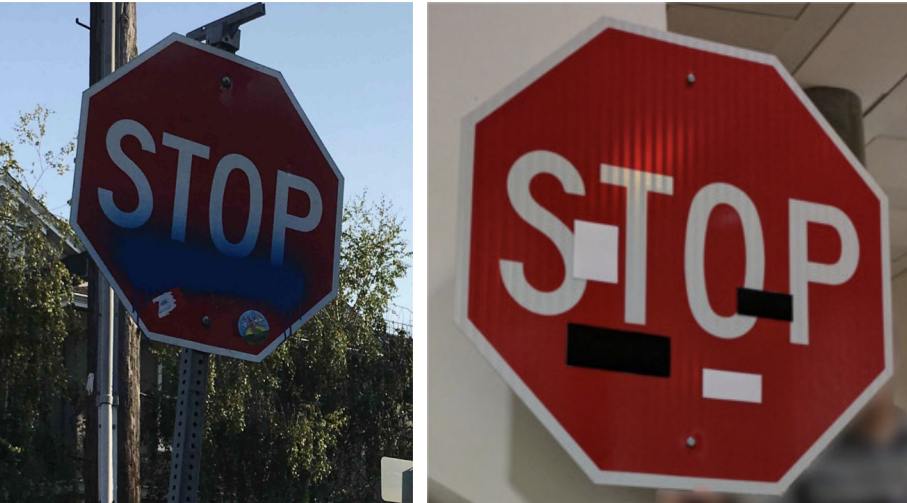
\includegraphics[width=0.46\linewidth]{figure/AEstop.png}\quad 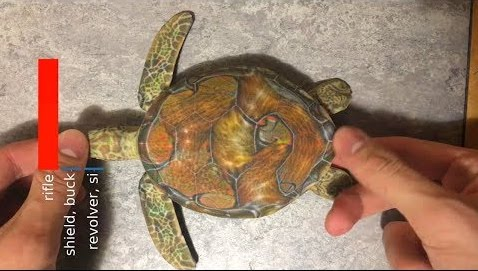
\includegraphics[width=0.45\linewidth]{figure/AEturtle.jpg}
  \label{fig:mnist}
\end{figure} 

\begin{columns}[totalwidth=\textwidth]

\begin{column}{0.5\textwidth}

\begin{itemize}
    \item Stop signs can be missclassified\\ e.g., because of graffiti
    \item With some well-placed patches, the model identifies it as a ``right of way'' sign
\end{itemize}

\end{column}

\begin{column}{0.5\textwidth}

\begin{itemize}
    \item 3D-print of a turtle
    \item Misclassified as a rifle (from every angle)
    \item Video: 
    \citebutton{MITCSAIL
    (2017)}{https://www.youtube.com/watch?v=piYnd_wYlT8}
\end{itemize}

\end{column}

\end{columns}


\end{vbframe}

\begin{vbframe}{Example: Tabular Data \citebutton{Ballet (2019)}{https://arxiv.org/pdf/1911.03274.pdf}}
What is imperceptibility on tabular data?
\begin{itemize}
    \item Idea: experts focus on the most important features in their judgment
    \item An ADE arises from manipulating features the model deems important but experts do not
\end{itemize}
\begin{figure}[h]
\centering
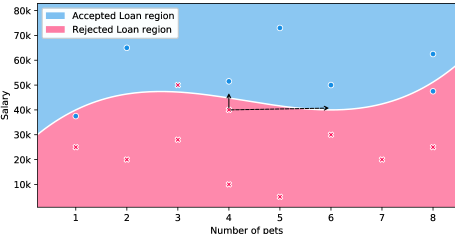
\includegraphics[width=0.6\linewidth]{figure/AEloanApplication.png}\\
   \centering
  {Decision boundary of a classifier deciding loan applications. ADE via ``number of pets''}
  \label{fig:mnist}
\end{figure} 

\end{vbframe}

\begin{vbframe}[c]{ADE and Interpretability}

\begin{enumerate}
    \item ADEs show where models fail $\leadsto$ improved model understanding
    \item Because of ADEs, we need more interpretability
    \item Interpretation can lead to robustness against ADEs
    \medskip
    \item Explanations can be used to construct ADEs (e.g., see numer of pets on previous slide)
\end{enumerate}

\end{vbframe}

\begin{vbframe}[c]{Formal Definition}
\begin{block}{Adversarial Input}
Let $\epsilon>0$, $f:\Xspace \rightarrow \Yspace$ be an ML model and $\xv \in \Xspace$ be a real data point that is correctly classified: $f(\xv)=y_{\xv,true}$. \\\medskip
 We call $\mathbf{a}_{\xv}$ an \textbf{adversarial input} to $\xv$ if:
\begin{equation*}
    \| \mathbf{a}_{\xv}- \xv\|<\epsilon\text{ and } f(\mathbf{a}_{\xv})\neq y_{\mathbf{a}_{\xv},true}=f(\xv)
\end{equation*}
\end{block}
\begin{itemize}
    \item $\mathbf{a}_{\xv}$ an is a data point close to a real, correctly classified input that is misclassified
    \item $\mathbf{a}_{\xv}$ is called \textbf{targeted} if the class it is assigned to is determined\\
    $f(\mathbf{a}_{\xv})=y'$ with $y'$ being a desired prediction
    \item Can be generalized to regression problems
\end{itemize}
\end{vbframe}


% \begin{vbframe}{ADE and Counterfactual Explanations}
% It seems as if ADEs and counterfactual explanations (CEs) are defined similarly. Both ADEs and CEs describe inputs close to a given input $\xv$ that gets a different assignment. What are their differences?
% \begin{itemize}
%     \item Counterfactuals do not have to be misclassified.
% %    \item Counterfactuals should be maximally close to $\xv$.
%     \item Different notions of distance $\|\cdot\|$ are applied, e.g., $p_{2,\infty}$-norm for ADEs or $p_{0,1}$-norm for CEs.
%     \item Informal difference I: ADEs are mostly considered for high-dimensional data, while CEs are mostly considered in the context of low-dimensional data.
%     \item Informal difference II: ADEs hide changes while CEs highlight them.
%     \item \textbf{Shared example:} ``If you had two more pets, your loan application would have been granted" is an example of both ADEs and CEs.
% \end{itemize}
% \end{vbframe}


\begin{frame}{Why Do ADE Exist?}
Non-exhaustive list of hypotheses: \\[0.5cm]
    
\only<1>{
    \textbf{1. Low-probability spaces hypotheses:} ADEs live in low-probability yet dense spaces in the data manifold that are not well represented in the training samples \citebutton{Szegedy et al. (2013)}{https://arxiv.org/abs/1312.6199}
        
    \begin{figure}
        \centering
        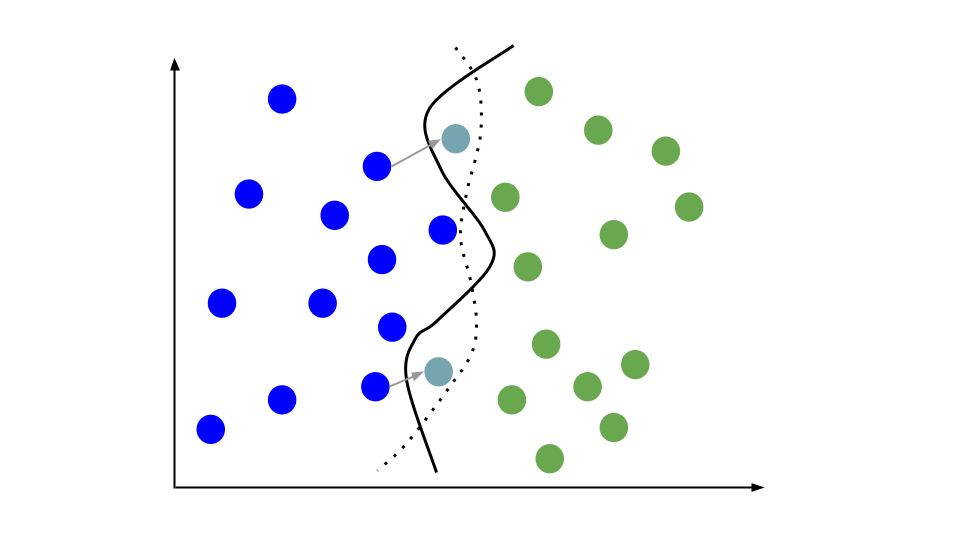
\includegraphics[width = .5\textwidth]{figure/adversarial examples.png}
        \caption{Binary classification example (dark blue vs. green dots). Dotted line represents the true decision boundary, bold line the trained one. Low probability space close to decision boundary allow for adversarial examples (turquoise dot).}
    \end{figure}
}
    
\only<2>{
    \textbf{2. Linearity hypotheses (most popular):}\\ Adversarial examples are omnipresent in the data manifold\\
    $\leadsto$ occur, because commonly used models often show linear behavior\\
    $\leadsto$ small changes of $\epsilon$ in every feature cause a change of $\epsilon\|\thetab\|_1$ in prediction \citebutton{Goodfellow et al. (2014)}{https://arxiv.org/abs/1412.6572}

    \vspace{.5cm}
    
    \textbf{Example:} linear model
    
    Original: $f(\xv) = \xv^T \thetab$ 
    
    Small changes: $f(\xv + \epsilon) = (\xv + \epsilon)^T \thetab$
    
    Difference: $f(\xv + \epsilon) - f(\xv) = \epsilon \cdot \thetab$
}
    
\only<3>{
    \textbf{3. The boundary tilting hypothesis:} Linearity is neither necessary nor sufficient to explain ADEs\\
    $\leadsto$ ADEs mostly result from overfitting the sampled manifold \citebutton{Tanay and Griffin (2016)}{https://arxiv.org/abs/1608.07690}
    
    \begin{figure}
        \centering
        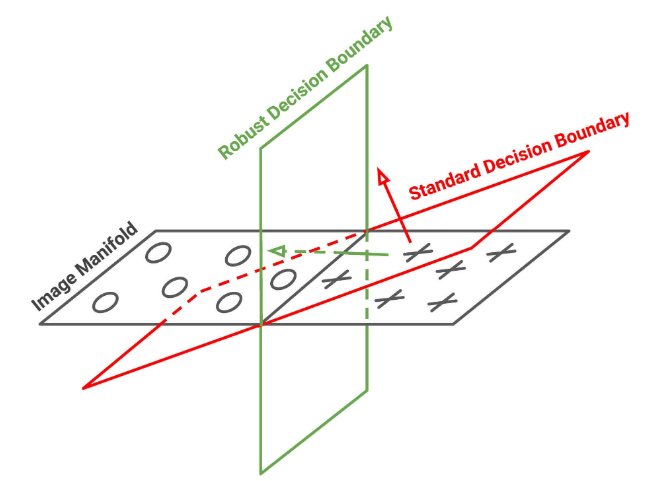
\includegraphics[width = .35\textwidth]{figure/tilting_ae.png}
        \caption{Linear binary classification example. Due to overfitting the decision boundary (red) is close to the manifold of the training data. Techniques like regularization could help to make the decision boundary more robust (green). \citebutton{Kim et al. (2019)}{https://arxiv.org/abs/1903.11626}
}
    \end{figure}
}
    
\only<4>{
    \textbf{4. Human-centric hypotheses:} ML models make use of predictive but non-robust features -- meaning they are highly correlated with the prediction target, but not used by humans \citebutton{Ilyas et al. (2019)}{https://papers.nips.cc/paper/2019/hash/e2c420d928d4bf8ce0ff2ec19b371514-Abstract.html}
}
    
\end{frame}


\begin{vbframe}[c]{Ways to Generate ADE}
Different ways for constructing ADEs:
There exist various ways in the literature to generate ADEs for a given model in feasible time
\begin{itemize}
    \item Formulate the search for ADEs as an \textbf{optimization problem}, e.g. 
    \begin{equation*}
        \label{eq:optimization}
        \underset{\xv'\in \Xspace}{\text{argmin}}\; \underbrace{\| \xv-\xv' \|_{\Xspace}}_{\text{minmize}} - \lambda\;   \underbrace{ \|f(\xv')-y'\|_{\Yspace}}_{\text{maximize}}
    \end{equation*}
    \item Use \textbf{sensitivity analysis} to identify features that influence the target class
    \item Train a generative adversarial network (GAN) \citebutton{Goodfellow et al. (2014)}{https://papers.nips.cc/paper/2014/file/5ca3e9b122f61f8f06494c97b1afccf3-Paper.pdf}
\end{itemize}
Moreover, depending on the attacker's model access, we can distinguish between
\begin{itemize}
    \item \textbf{Full-access attacks}: the attacker has full access to the internals of the model
    \item \textbf{Black-box attacks}: the attacker can only query the model on some inputs and receives the model's outputs
\end{itemize}
\end{vbframe}

\begin{vbframe}{Fast-Gradient-Sign-Method (FGSM)
\citebutton{Goodfellow et al. (2015)}{https://arxiv.org/pdf/1412.6572.pdf}}
% Since we have seen optimization methods for CEs, we focus on a method using sensitivity analysis, namely FGSM.
% Source of (modified) figure: https://docs.google.com/presentation/d/1l-ng618qrisSorutii9I30qL8VhZGYD9aRBuwvvBbSY/edit?usp=sharing
\begin{itemize}
    \item FGSM is based on the linearity hypothesis
    \item FGSM finds ADEs from:
    \begin{equation*}
        a_{\xv}=\xv+\epsilon\cdot\text{sign}(\nabla_{\xv} J(\theta,\xv,y_{\xv,true}))
    \end{equation*}
    where $\text{sign}(\nabla_{\xv} J(\theta,x,y_{\xv,true}))$ describes the component-wise signum of the gradient of cost function $J$ in $\xv$ with true label $y_{\xv,true}$
\end{itemize}
\begin{figure}[h]
\centering
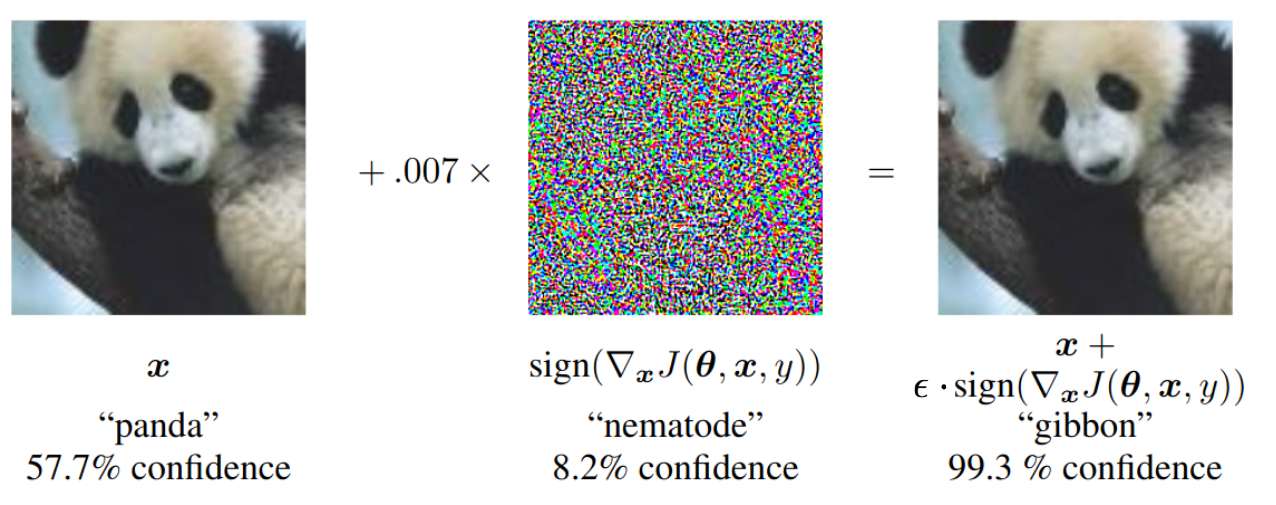
\includegraphics[width=0.7\linewidth]{figure/AEpanda.png}
  \label{fig:mnist}
\end{figure} 

\end{vbframe}

\begin{vbframe}[c]{Notes on FGSM \citebutton{Goodfellow et al. (2015)}{https://arxiv.org/pdf/1412.6572.pdf} \citebutton{Lyu et al. 2015}{https://arxiv.org/abs/1511.06385}}
\begin{itemize}
    \item FGSM works particularly well for linear(-like) models in high-dimensional spaces,\\ e.g., LSTMs, logistic regressions or CNNs with ReLU activations
    \item Not every $\mathbf{a}_{\xv}$ generated by FGSM is an ADE, especially if $\epsilon$ is too small
    \item FGSM attacks can be also generated without model access by approximating the gradient,\\ e.g. with finite difference methods
    \item The notion of similarity in FGSM is based on $\|\cdot\|_{\infty}$ $\leadsto$ there are generalizations of FGSM to other norms
\end{itemize}
\end{vbframe}


\begin{vbframe}[c]{Black-Box Attacks with Surrogates \citebutton{Papernot et al. (2016)}{https://arxiv.org/abs/1605.07277}}

\begin{itemize}
    \item So far, we assumed full access to the predictive model
    \item Black-box attacks only assume query-access
    \item Large risk of attacks since often one can query predictive models many times
\end{itemize}

\medskip
\begin{enumerate}
    \item Query the model you aim to attack as often as allowed on data similar to the training data
    \item Use the labeled data you received to train a surrogate model
    \item Generate ADEs for the surrogate model
    \item Use these ADEs to attack the original model
\end{enumerate}

\medskip
\begin{itemize}
    \item[$\leadsto$] Known as the \textbf{transferability} of ADEs.
\end{itemize}



\end{vbframe}

\begin{vbframe}[c]{Defenses Against ADE}
There are several ways to protect your network against such attacks -- we distinguish between two broad types of defenses, differing in the position in which they act
\begin{itemize}
    \item \textbf{Guards} act on the inputs a model receives
    \begin{itemize}
        \item \textbf{Detect anomalies:} e.g., statistical testing, or discriminator networks from GANs
        \item \textbf{Conduct transformations} on inputs (e.g. PCA)
    \end{itemize}
    \item \textbf{Defense by design} act on the model itself
    \begin{itemize}
        \item \textbf{Adversarial training}: train model on adversarials
        \item \textbf{Architectural defenses}: e.g., removing low predictive features from the model
    \end{itemize}
\end{itemize}
\end{vbframe}

%\begin{vbframe}{Regularization Against ADEs}
%The use of regularization techniques against ADEs is motivated by most hypotheses that explain ADEs. As an example we look at a technique based on the FGSM and the linearity hypotheses.
%\begin{itemize}
%    \item Goodfellow et al. suggest to specfiy the cost function s.t.
%    \begin{equation*}
%        \tilde{J}(\theta,\xv,y):=\alpha J(\theta,\xv,y)+(1-\alpha) J(\theta,\xv+\epsilon\cdot\text{sign}(\nabla_{\xv} J(\theta,\xv,y)),y)
%    \end{equation*}
%    with $\alpha=0.5$.
%    \item This increased the model robustness against FGSM generated ADEs.
%    \item However, model are not only still prone to other ADEs but also to many FGSM-ADEs.
%    \item Applying such regularization terms can increase test error.
%\end{itemize}
%\end{vbframe}

\begin{vbframe}[c]{Summary}
\begin{itemize}
    \item ADEs are not explanations themselves but are conceptually connected to them
    \item ADEs can be generated in diverse settings $\leadsto$ crucial modeling decisions are the distance measure, the local environment, and the target level (model or process)
    \item There are various hypotheses on the existence of ADEs which also motivate different defense strategies
\end{itemize}
\begin{center}
    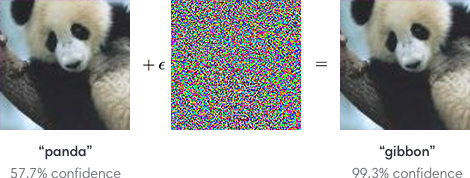
\includegraphics[width = .6\textwidth]{figure/AEpanda_simple.png}
    
    {\citebutton{Goodfellow et al. (2017)}{https://openai.com/blog/adversarial-example-research/}}
\end{center}
\end{vbframe}

%\begin{vbframe}{Outlook}
%\begin{itemize}
%    \item Even in highly non-linear models ADEs occur. As long as their existence is not well-understood, defenses against them will have limited power.
%    \item More and more different distance measures are considered, e.g. $p_0$ for one-pixel attacks, the Wasserstein-metric or psychologically motivated measures like the Perceptual Adversarial Similarity Score (PASS).
%    \item Recent work considered ADEs that fool both, humans and ML models. ADEs may be a case where research on human and machine perception can profit from each other.
%\end{itemize}
%@misc{rozsa2016adversarial,
%      title={Adversarial Diversity and Hard Positive Generation}, 
%      author={Andras Rozsa and Ethan M. Rudd and Terrance E. Boult},
%      year={2016},
%      eprint={1605.01775},
%      archivePrefix={arXiv},
%      primaryClass={cs.CV}
%}
%\end{vbframe}

% \begin{vbframe}{Central References}
% \begin{itemize}
%     \item Serban, A., Poll, E., \& Visser, J. (2020). Adversarial examples on object recognition: A comprehensive survey. ACM Computing Surveys (CSUR), 53(3), 1-38.
%     \item Goodfellow, I. J., Shlens, J., \& Szegedy, C. (2014). Explaining and harnessing adversarial examples. arXiv preprint arXiv:1412.6572.
%     \item Yuan, X., He, P., Zhu, Q., \& Li, X. (2019). Adversarial examples: Attacks and defenses for deep learning. IEEE transactions on neural networks and learning systems, 30(9), 2805-2824.
% \end{itemize}
% \end{vbframe}

\endlecture
\end{document}
